\chapter{Richiami di Teoria delle probabilità} 

\begin{figure}[h]
    \centering
    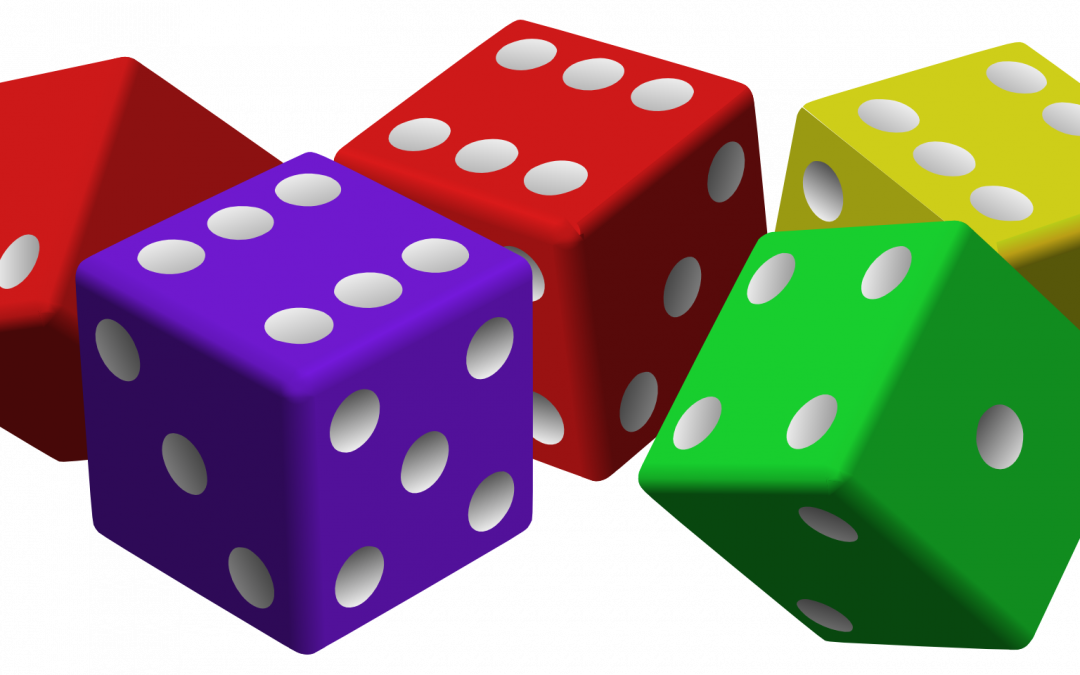
\includegraphics[scale = 0.4]{dadi.png}
\end{figure} 

\newpage 

\begin{tcolorbox}
Questo capitolo è da sapere come l'Ave Maria, perchè è l'argomento più importante di questo corso. \newline 
Se non sapete questo, è meglio non presentarsi all'orale.     
\end{tcolorbox}

\section{Cosa è una variabile aleatoria} 

Classificando i segnali, all'inizio del corso, si è fatta distinzione tra segnali determinati e segnali aleatori. \newline 

Cominciamo con il ricordare la definizione di esperimento aleatorio: 
si definisce un "evento" di qualunque natura e consistenza il cui risultato non è certo a priori ma, 
può assumere una serie di esiti caratterizzati da un valore di probabilità. \newline 

Consideriamo un segnale aleatorio riguardo un esperimento aleatorio. \newline 

Un segnale del tipo

{
    \Large 
    \begin{equation}
        s(t) = A \cos(2 \pi f_0 t +\phi)
    \end{equation}
}

ha diverse variabili: 

\begin{itemize}
    \item A (che indica l'ampiezza) e $f_0$ (frequenza) sono quantità determinate 
    \item $\phi$ può assumere, con la stessa probabilità, un qualunque valore compreso tra $0$ e $2\pi$ 
\end{itemize}

Quindi, il valore di $\phi$ può assumere diverso ogni volta. \newline 

In questo caso $\phi$ prende il nome di variabile aleatoria. \newline 

La variabile aleatoria può essere: 
\begin{itemize}
    \item discreta, quando l'insieme dei valori che essa assume è discreto 
    \item continua, quando l'insieme dei valori che essa assume è continuo
\end{itemize}

Se consideriamo l'esperimento del lancio del dado, i risultati dell'esperimento, cioè le facce del dado, sono aleatori discreti, 
invece, la variabile $\phi$ del segnale s(t) è una variabile aleatoria continua compresa tra $0$ e $2\pi$. \newline 

In altri casi, si hanno variabili aleatorie miste, in cui alcuni valori (discreti) sono più importanti degli altri. \newline 

Spesso, a livello di notazione, per indicare la variabile aleaotoria si utilizzano le lettere maiuscole, 
mentre le lettere minuscole stanno ad indicare un particolare esito dell'esperimento aleatorio (si parla di realizzazione o determinazione). \newline 

Quindi, nell'equazione del segnale s(t) citato precedentemente, è più appropriato indicare $\phi$ come $\Phi$: 

{
    \Large 
    \begin{equation}
        \begin{cases}
            s(t) = A \cos(2 \pi f_0 t +\phi) \\ 
            \phi = \Phi 
        \end{cases} 
        \Rightarrow 
        s(t) = A \cos(2 \pi f_0 t +\Phi)
    \end{equation}
} 

Invece se indichiamo $\phi$ con la lettera minuscola, significa che la variabile aleatoria ha assunto il particolare valore $\phi$. \newline 

Quindi, possiamo intuire che, la singola variabile aleatoria è associata un numero il quale esprime la probabilità che si ottenga proprio quel valore come risultato dell'esperimento. \newline 

\newpage 

\subsection{Cosa è un evento} 

Oltre che i singoli risultati di un esperimento, è spesso importante considerare dei gruppi di risultati. \newline 

Consideriamo l'esperimento aleatorio che consiste nel contare il numero di persone che, in un ben determinato intervallo della giornata, si presentano alla cassa di un supermercato. \newline 

Questo è un esperimento aleatorio, in quanto, non è detto sapere a priori quale sarà tale numero. \newline 

Inoltre, si vuole considerare la probabilità che il numero di clienti nell'intervallo temporale considerato sia maggiore di 20. \newline 

L'interesse nell'esperimento potrebbe allora essere concentrato sul seguente evento: numero di clienti superiore a 20, nel qual caso i valori di interesse della variabile aleatoria, detta X, sarebbe solo quelli che soddisfano tale condizione. \newline 

Indicando dunque con $\Omega$ (la lettera greca $\Omega$ si legge Omega) l'insieme complessivo dei valori possibili (tale insieme si chiama spazio campione), 
gli eventi sono sottoinsime dello spazio campione che verificano le seguenti condizioni:

\begin{enumerate}
    \item se A è un evento, anche il suo complemento $\overline{A}$ rispetto all'insieme $\Gamma$, è un evento 
    \item se A e B sono eventi, anche la loro unione $A \cup B$ è un evento 
    \item se A e B sono eventi, anche la loro intersezione $A \cap B$ è un evento 
    \item dato un evento A, gli insiemi $A \cup \overline{A}$ e $A \cap \overline{A}$ sono particolari eventi 
    \begin{enumerate}
        \item $A \cup \overline{A}$ , che coincide con $\Omega$ (ovvero con lo spazio campione), è detto evento certo 
        \item $A \cap \overline{A}$ , che coincide con $\emptyset$ e non contiene alcun risultato dell'esperimento, è detto evento impossibile
    \end{enumerate}
\end{enumerate} 

\newpage 

\section{Teoria assiomatica di Kolmogorov}

Assegnato un esperimento aleatorio con uno spazio comune $\Omega$ e l'insieme degli eventi ad esso relativi, 
detto classe degli eventi ed indicato con S, una legge di probabilità $ \Pr{\cdot} $ è una corrispondenza che associa ad ogni elemento di S, e quindi ad ogni evento di interese in una prova dell'esperimento, 
un numero reale che soddisfa i seguenti assiomi (cioè enunciati che non hanno bisogno di dimostrazione): 

\begin{enumerate}
    \item la probabilità di un evento arbitrario A è non negativa, si ha cioè: 
    {
        \Large 
        \begin{equation}
            \Pr{A} \geq 0
        \end{equation}
    }

    \item la probabilità dell'evento certo è unitaria (assioma di normalizzazione), si ha cioè: 
    {
        \Large 
        \begin{equation}
            \Pr{\Omega} = 1
        \end{equation}
    } 

    \item dati due eventi A e e B mutuamente esclusivi 
    (ovvero incompatibili, cioè tali che non possano verificarsi contemporaneamente) la probabilità dell'evento unione è data dalla somma delle probabilità dei singoli eventi, si ha cioè: 
    {
        \Large 
        \begin{equation}
            A \cup B = \emptyset 
            \rightarrow 
            \Pr{A \cup B} = \Pr{A} + \Pr{B}
        \end{equation}
    }
\end{enumerate}

Da questi assiomi, si ricavano le seguenti proprietà: 

\begin{itemize}
    \item dato un evento A, la probabilità dell'evento complementare $\overline{A}$ è data dal complemento a 1 della $\Pr{A}$, si ha cioè:
    {
        \Large 
        \begin{equation}
            \Pr{\overline{A} } = 1 - \Pr{A}
        \end{equation}
    }

    \item l'insieme impossibile ha la proprietà nulla di verificarsi, si ha cioè: 
    {   
        \Large 
        \begin{equation}
            \Pr{\emptyset} = 0    
        \end{equation}
    }

    \item la probabilità di un evento A non può assumere valore maggiore di 1, si ha cioè: 
    {
        \Large 
        \begin{equation}
            0 \leq \Pr{A} \leq 1
        \end{equation}
    } 

    \item dati due eventi A e B, la probabilità dell'evento unione $A \cup B$ è espressa dall'uguaglianza:
    {
        \Large 
        \begin{equation}
            \Pr{A \cup B} = \Pr{A} + \Pr{B} + \Pr{A \cap B}
        \end{equation}
    } 
\end{itemize}

Data una coppia di eventi A e B, la probabilità dell'evento intersezione, spesso indicata semplicemente con $\Pr{A, B}$, è detta probabilità congiunta, 
mentre $\Pr{A}$ e $\Pr{B}$ hanno il significato di probabilità marginali. \newline 

Data una coppia di eventi A e B con $\Pr{B} \neq 0$, si definisce poi la probabilità condizionata: 

{
    \Large 
    \begin{equation}
        \begin{split}
            \Pr{A | B} 
            &= 
            \frac{\Pr{A \cup B}}{\Pr{B}} 
            \\
            &= 
            \frac{\Pr{A, B}}{\Pr{B}}     
        \end{split}
    \end{equation}
} 

la quale esprime la probabilità dell'evento A condizionata al verificarsi dell'evento B (che ha dunque il significato di evento condizionante). \newline 

Utilizzando i diagrammi, possiamo capire meglio gli eventi. \newline 

\begin{figure}[h]
    \centering
    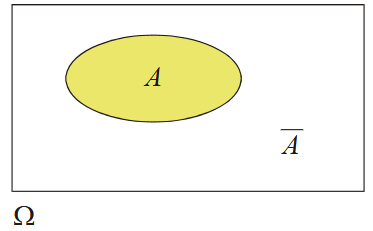
\includegraphics[scale = 0.6]{Evento A e il suo complementare.PNG}
\end{figure} 

\newpage

La figura ci mostra il rettangolo $\Omega$ che rappresenta l'evento certo, 
il cerchio giallo A rappresenta l'evento A, lo spazio bianco del rettangolo $\Omega$, cioè $\overline{A}$, rappresenta il complementare di A. \newline 

\begin{figure}[h]
    \centering
    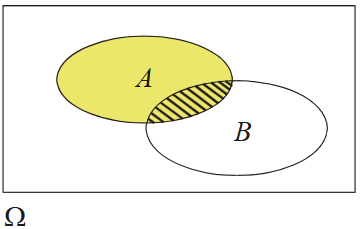
\includegraphics[scale = 0.6]{A unione B.PNG}
\end{figure} 

In questo caso, la figura dimostra l'evento $A \cup B$ ed è rappresentato dalla sovrapposizione dei diagrammi A e B; 
sommando, semplicemente, le $\Pr{A}$ e $\Pr{B}$, la probabilità di $A \cap B$ verrebbe conteggiata due volte. \newline 

\begin{figure}[h]
    \centering
    \includegraphics[scale = 0.6]{A unione B se A intersezione B è vuoto.PNG}
\end{figure} 

Se invece, come in figura, $A\cap B = \emptyset$, allora $\Pr{A \cup B} = \Pr{A} + \Pr{B}$. \newline 

\newpage 

\section{Definzione classica di probabilità}

In accordo con questa definizione storica attrubuita a Laplace, 
la $\Pr{A}$ si calcola: 

\begin{itemize}
    \item individuando il numero $N_F (A)$ dei cosiddeti casi favorevoli ad A 
    \item individuando il numero $N_P$ dei cosiddetti casi possibili 
    \item dividendo $N_F (A)$ per $N_P$
\end{itemize}


In formula: 

{
    \Large 
    \begin{equation}
        \Pr{A} = \frac{N_F (A)}{N_P}
    \end{equation}
}

In pratica: $N_P$ è il numero totale dei risultati contenuti in $\Omega$, mentre $N_F (A)$ è il numero di risultati contenuti in A. \newline

Se esiste l'equiprobabilità di un evento, allora possiamo utilizzare la definizione anche pratica oltre a quella classica. \newline 

Se non esiste l'equiprobabilità, ad esempio in un dado truccato, non si può utilizzare la definzione classica di probabilità. \newline 

\newpage 

\section{Definizione frequentistica di probabilità di Von Mises}

Questa definizione è simile a quella classica, ma ha il vantaggio di poter essere applicata anche nel caso di esperimento non simmetrico (cioè, in senso pratico, anche in un dado truccato). \newline 

Si esprime la probabilità come un rapporto, ma, in questo caso, 
le quantità a numeratore e denominatore sono ricavate sperimentalmente. \newline 

Per poter calcolare la $\Pr{A}$ nel caso sperimentale: 

\begin{itemize}
    \item si ripete l'esperimento aleatorio di un evento A 
    \item si conta il numero di volte $N_A$ in cui l'esperimento ha dato un esito favorevole ad A 
    \item si divide $N_A$ per N
\end{itemize}


Il punto rilevante è che il rapporto così ottenuto approssima la probabilità di errore corretta solo a patto di considerare un numero di ripetizioni dell'esperimento sufficientemente elevato 
(al limite tende all'infinto). \newline 

Si deve imporre: 

{
    \Large 
    \begin{equation}
        \Pr{A} = \lim_{N \rightarrow \infty} \frac{N_A}{N}
    \end{equation}
}

Il passaggio al limite resta, essenzialmente, un'astrazione matematica, ragion per cui non sono rari i casi in cui l'uso della $\Pr{A}$ definita adesso fornisce solo un'approssimazione della probabilità cercata. \newline 

Ovviamente, nei casi in cui si è convinti della simmetria dell'esperimento, e dunque dell'equiprobabilità dei risultati, 
è conveniente ed opportuno l'uso della definizione classica di probabilità, assai più semplice da calcolare. \newline 


È anche importante evidenziare che, la definizione frequentistica non è in contrasto con quella assiomatica di Kolmogorov. \newline 

Infatti, la probabilità $\Pr{A}$ espressa adesso è: 

\begin{itemize}
    \item una quantità non negativa, poichè tradotta dal limite di un rapporto fra quantità positive 
    \item se l'evento A coincide $\Omega$, allora, banalmente, si ha $N_A = N$ e quindi $\Pr{A} = 1$
    \item se A e B sono due eventi che si escludono vicedevolmente (si dice mutualmente esclusivi), allora una prova dell'esperimento verificare $A \cup B$ dà un risultato che sta in A o in B, 
    ma, che, non può stare in entrambi: ne consegue che $N_{A \cup B} = N_A + N_B$ e quindi 
    {
        \Large 
        \begin{equation}
            \begin{split}
                \Pr{A \cup B} 
                &= 
                \lim_{N \rightarrow \infty} 
                \frac{N_{A \cup B}}{N} 
                \\ 
                &= 
                \lim_{N \rightarrow \infty} 
                \frac{N_A + N_B}{N} 
                \\ 
                &= 
                \lim_{N \rightarrow \infty} 
                \frac{N_A}{N} 
                + 
                \lim_{N \rightarrow \infty} 
                \frac{N_B}{N} 
                \\ 
                &= 
                \Pr{A} + \Pr{B}
            \end{split}
        \end{equation}
    }
\end{itemize}

I tre assiomi della teoria assiomatica di Kolmogorov rimangono verificati, e con loro anche le proprietà. \newline 

\newpage 

\section{Eventi statisticamente indipendenti} 

Due eventi A e B sono indipendenti se il verificarsi dell'uno non ha alcuna implicazione sul verificarsi dell'altro. \newline 

Per eventi indipendenti: 

{
    \Large 
    \begin{equation}
        \Pr{A} = \Pr{A | B}
    \end{equation}
}

{
    \Large 
    \begin{equation}
        \Pr{B} = \Pr{B | A}
    \end{equation}
}

Ricordando la definizione di probabilità condizionata: 

{
    \Large 
    \begin{equation}
        \Pr{A | B} = \frac{\Pr{A, B}}{\Pr{B}}
    \end{equation}
} 

si può concludere che, per eventi indipendenti: 

{   
    \Large 
    \begin{equation}
        \Pr{A, B} = \Pr{A} \cdot \Pr{B}   
    \end{equation}
}

e cioè, che la probabilità congiunta è uguale al prodotto delle probabilità marginali (dei singoli eventi). \newline 

Un altro importante risultato è il teorema (o formula) di Bayes, che può essere formalizzato nel modo seguente: 

{
    \Large 
    \begin{equation}
        \Pr{A | B} = \frac{\Pr{B | A} \cdot \Pr{A}}{\Pr{B}}
    \end{equation}
} 

La formula di Bayes è spesso usata in combinazione con il teorema della probabilità totale, 
che esaminiamo di seguito. \newline 

\subsection{Teorema della probabilità totale} 

Costruiamo, preliminarmente, una partizione dello spazio $\Omega$ scegliendo N eventi $B_i$ (con $i = 1, 2, ..., N$) 
di S con le seguenti proprietà: 

{
    \Large 
    \begin{equation}
      B_i \cap B_k = \emptyset \text{ se } i \neq k   
    \end{equation}
}

{
    \Large 
    \begin{equation}
        \bigcup_{i = 1} ^{N} B_i = \Omega 
    \end{equation}
}

$B_i \cap B_k = \emptyset \text{ se } i \neq k$ esprime il fatto che, gli elementi della partizione sono disgiunti. \newline 

Invece $\bigcup_{i = 1} ^{N} B_i = \Omega$ esprime il fatto che l'unione di tutti gli eventi della partizione restituisce lo spazio comune. \newline 

Un esempio dal punto di vista grafico di quello che abbiamo scritto in formule: 

\begin{figure}[h]
    \centering
    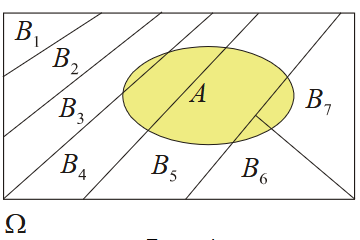
\includegraphics[scale = 0.6]{Formula di Bayes in pratica.PNG}
\end{figure} 

\newpage 

Nella stessa figura è anche rappresentato un generico evento A, che non è un elemento della partizione. \newline 

Ricordando l'assioma della teoria assiomatica di Kolmogorov: 

{
    \Large 
    \begin{equation}
        A \cup B = \emptyset 
        \rightarrow 
        \Pr{A \cup B} = \Pr{A} + \Pr{B}
    \end{equation}
}

allora possiamo scrivere: 

{
    \Large 
    \begin{equation}
        \begin{split}
            \Pr{A} 
            &= 
            \Pr{A \cup B} 
            \\ 
            &= 
            \Pr{A \cap \bigcup_{i =1}^{N} B_i}
            \\ 
            &= 
            \Pr{\bigcup_{i =1}^{N} A \cap B_i}
            \\ 
            &= 
            \sum_{i = 1}^{N}
            \Pr{A \cap B_i} 
            \\ 
            &= 
            \sum_{i = 1}^{N}
            \Pr{A | B_i} \cdot \Pr{B_i} 
        \end{split}
    \end{equation}
}

Quindi dalla formula di Bayes del tipo: 

{
    \Large 
    \begin{equation}
        \Pr{A | B} = \frac{\Pr{B | A} \cdot \Pr{A}}{\Pr{B}}
    \end{equation}
}

con un cambio di notazione, possiamo riscrivere la formula di Bayes come: 

{
    \Large 
    \begin{equation}
        \Pr{B_i | A} = \frac{\Pr{A | B_i} \cdot \Pr{B_i}}{\Pr{A}}
    \end{equation}
}

Inoltre, grazie alla nuova formula di $\Pr{A}$ che abbiamo trovato, cioè 
$\Pr{A} = \sum_{i = 1}^{N} \Pr{A | B_i} \cdot \Pr{B_i}$, possiamo riscrivere $\Pr{B_i | A}$ come: 

{
    \Large 
    \begin{equation}
        \Pr{B_i | A} = \frac{\Pr{A | B_i} \cdot \Pr{B_i}}{\sum_{i = 1}^{N} \Pr{A | B_i} \cdot \Pr{B_i}}  
    \end{equation}
}

che è, in effetti, la formula ampiamente utilizata nella pratica. \newline 

\newpage 

\section{Esperimento di Bernoulli} 

Un esperimento aleatorio di grande importanza nella pratica è quello delle prove di Bernoulli (o prove ripetute binarie e indipendenti). \newline 

Si definisce tale un esperimento aleatorio a due soli esiti, indicati con $x_1$ e $x_2$ caratterizzati da: 

{
    \Large 
    \begin{equation}
        \Pr{x_1} = p
    \end{equation}
}

{
    \Large 
    \begin{equation}
        \begin{split}
            \Pr{x_2} = q = 1 - p    
        \end{split}
    \end{equation}
}

Si considerano n ripetizioni dell'esperimento assicurandosi che la singola ripetizione non abbia alcuna relazione con le altre (ipotesi di indipendenza) 
e si considera l'evento: 

{
    \Large 
    \begin{equation}
        A = {x_1}
    \end{equation}
}

in cui $x_1$ si è presentato k volte nelle n prove ripetute. \newline 

In virtù dell'indipendenza, applicando ripetutamente il risultato 

{
    \Large 
    \begin{equation}
        \Pr{A, B} = \Pr{A} \cdot \Pr{B}
    \end{equation}
}

all'evento A ed il suo complementare $\overline{A}$, si trova immediatamente: 

{
    \Large
    \begin{equation}
        \begin{split}
            \Pr{A} 
            &= 
            \binom{n}{k} 
            p^{k} 
            q^{n - k} 
            \\ 
            &=
            \frac{n!}{k! (n-k)!}
            p^{k} 
            (1-p)^{n-k}    
        \end{split}
    \end{equation}
}

Questa formula è definita come formula di Bernoulli. \newline 

Il termine $p^{k} q^{n-k}$ esprime il fatto che sono favorevoli all'evento A i casi in cui $x_1$ 
si è presentato k volte e, conseguentemente, $x_2$ si è presentato $(n-k)$ volte, 
mentre il coefficiente binomiale $\binom{n}{k}$ tiene conto del numero di tali casi, 
potendosi disporre, nella sequenza delle repliche dell'esperimento, i k valori $x_1$ in un numero di modi che uguaglia le combinazioni semplici di classe 
k di n elementi. \newline 

\newpage 

\section{Distribuzione di probabilità cumulativa e densità di probabilità} 

In molti contesti di interesse pratico, si pone il problema di calcolare la probabilità che una variabile aleatoria X 
assuma valori all'interno di un dato intervallo $(a, b]$, vale a dire la 
$\Pr{a < X \leq b}$. \newline 

Con la notazione $(\cdot , \cdot ]$ si indica un intervallo aperto a sinistra e chiuso a destra. \newline 

Per una variabile qualsiasi posta in questo intervallo, possiamo definire la distribuzione di probabilità cumulativa (o funzione di ripartizione): 

{
    \Large 
    \begin{equation}
        F_X (x) = \Pr{X \leq x}
    \end{equation}
}

$F_X (x)$ esprime dunque la probabilità che la variabile aleatoria X assuma valori non maggiori del valore x assegnato. \newline 

$F_X (x)$ deve soddisfare le seguenti proprietà: 

\begin{enumerate}
    \item assume valori appartenenti all'intervallo [0, 1], cioè:
    {
        \Large 
        \begin{equation}
            0 \leq F_X (x) \leq 1
        \end{equation}
    }

    \item il suo valore limite per $x \rightarrow +\infty$ è uguale a 1, cioè: 
    {
        \Large 
        \begin{equation}
            \begin{split}
                \lim_{x \rightarrow +\infty} 
                F_X (x) 
                &= 
                F_X (+\infty) 
                \\ 
                &= 
                \Pr{X \leq +\infty} 
                \\ 
                &= 
                1
            \end{split}
        \end{equation}
    } 

    \item il suo valore limite per $x \rightarrow -\infty$ è uguale a 0, cioè: 
    {
        \Large 
        \begin{equation}
            \begin{split}
                \lim_{x \rightarrow -\infty} 
                F_X (x) 
                &= 
                F_X (-\infty) 
                \\ 
                &= 
                \Pr{X \leq -\infty} 
                \\ 
                &= 
                0
            \end{split}
        \end{equation}
    }

    \item è monotona non decrescente, cioè: 
    {
        \Large 
        \begin{equation}
            x_2 > x_1 \Rightarrow F_X (x_2) \geq F_X (x_1)
        \end{equation}
    } 

    \item se presenta una discontinuità di prima specie (cioè in quel punto si ha un salto e il limite destro e sinistro sono finiti ma diversi tra loro), 
    nel punto $x = \overline{x}$, allora la differenza tra il suo limite destro e il suo limite sinistro, 
    in tale punto è pari alla probabilità dell'evento $X = \overline{x}$, cioè: 
    
    {
        \Large 
        \begin{equation}
        \Pr{X = \overline{x}} 
        = 
        F_X(\overline{x}^{+})
        - 
        F_X(\overline{x}^{-})
        \end{equation}
    }

    avendo indicato con $F_X(\overline{x}^{+})$ il limite destro  
    e con $F_X(\overline{x}^{-})$ quello sinistro.
\end{enumerate}

La seconda proprietà deriva dal fatto che l'evento $X \leq +\infty$ coincide con l'evento certo $\Omega$. \newline 

Dualmente, la terza proprietà deriva dal fatto che l'evento $X \leq - \infty$ coincide con l'evento impossibile $\emptyset$. \newline 

Utilizzando la definizione di $F_X (x)$, è chiaro che si può scrivere: 

{
    \Large 
    \begin{equation}
        \begin{split}
            \Pr{a < X \leq b} 
            &= 
            \Pr{X \leq b} 
            - 
            \Pr{X \leq a} 
            \\
            &= 
            F_X (b) - F_X (a)
        \end{split}
    \end{equation}
}

Questa formula, risolve il probelma su come calcolare la probabilità di $\Pr{a < X \leq b} $. \newline 

Quindi il calcolo di $\Pr{a < X \leq b} $ può essere risolto utilizzando un'altra funzione denominata come 
funzione densità di probabilità. \newline 

La funzione di densità di probabilità è legata alla distribuzione di probabilità cumulativa con la seguente legge: 

{
    \Large 
    \begin{equation}
        f_X (x) = \frac{d F_X (x)}{d x}
    \end{equation}
}


Da questa relazione, possiamo scrivere la relazione inversa: 

{
    \Large 
    \begin{equation}
        F_X (x) 
        = 
        \int_{-\infty}^{x} 
        f_X (\xi) d\xi 
    \end{equation}
}

Anche la densità di probabilità deve soddisfare alcune proprietà; in particolare:

\begin{enumerate}
    \item è una funzione non negativa, cioè: 
    {
        \Large 
        \begin{equation}
            f_X (x) \geq 0
        \end{equation}
    } 

    \item  il suo integrale esteso all'interno dell'asse reale è uguale a 1, cioè: 
    {
        \Large 
        \begin{equation}
            \int_{-\infty}^{+\infty} 
            f_X (x) dx = 1
        \end{equation}
    }
\end{enumerate}

L'ultima proprietà viene definita anche come condizione di normalizzazione. \newline 

Inoltre, costituisce il primo passo fondamentale per verificare se una funzione può rappresentare o meno una densità di probabilità. \newline 

Utilizzando i grafici: 

\begin{figure}[h]
    \centering
    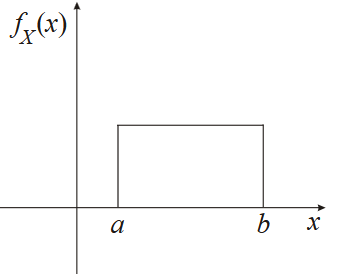
\includegraphics[scale = 0.6]{funzione densità di probabilità.PNG}
\end{figure} 

l'area del rettangolo deve essere uguale a 1, inoltre, se consideriamo l'intervallo delle x tra a e b, allora l'altezza sarà $\frac{1}{b - a}$. \newline 

Utilizzando la $f_X (x)$, la $\Pr{a < X \leq b}$ può anche essere calcolata come: 

{
    \Large 
    \begin{equation}
        \begin{split}
            \Pr{a < X \leq b} 
            &= 
            F_X (b) - F_X (a)
            \\ 
            &= 
            \int_{- \infty}^{b}
            f_X (x) dx 
            - 
            \int_{- \infty}^{a}
            f_X (x) dx 
            \\ 
            &= 
            \int_{a}^{b}
            f_X (x) dx 
        \end{split}
    \end{equation}
}

\newpage 

\section{Distribuzione di probabilità cumulativa nel dettaglio} 

All'inizio della trattazione si è detto che una variabile aleatoria può essere: 

\begin{itemize}
    \item discreta, quando l'insieme dei valori che essa assume è discreto 
    \item continua, quando l'insieme dei valori che essa assume è continuo 
\end{itemize}

Per come sono definite, la distribuzione di probabilità cumulativa e la densità di probabilità sembrano "naturalmente" 
adattarsi al caso di variabile continua.\newline 

Per quanto riguarda la distribuzione di probabilità cumulativa, si tratta di una funzione che rimane costante nei tratti che separano due generici valori possibili, e che si incrementa in corrispondenza 
di ciascuno di questi valori, per una quantità pari alla probabilità che lo caratterizza. \newline 

Un esempio di probabilità cumulativa: 

\begin{figure}[h]
    \centering
    \includegraphics[scale = 0.6]{Grafico di una distribuzione di probabilità cumulativa.PNG}
\end{figure} 

Generalizzando, la distribuzione di probabilità cumulativa per una variabile discreta è una funzione a 
gradini (costante a tratti), esprimibile come segue: 

{
    \Large 
    \begin{equation}
        F_X (x) 
        = 
        \sum_{k} 
        \Pr{X = x_k} 
        u(x - x_k)
    \end{equation}
}

dove gli $x_k$ sono i valori possibili e $u (x - x_k)$ è il gradino unitario che parte da $x_k$. \newline 

\begin{tcolorbox}
    Con la notazione $\sum_{k}$ si inendono tutti i possibili k disponibili, viene usata come notazione generale
\end{tcolorbox}

Per quanto riguarda la densità di probabilità di una variabile aleatoria discreta, essa, in senso stretto, 
sembrerebbe non definibile, visto che la formula di $F_X (x)$ appena citata non è derivabile. \newline 

Ma, grazie alla Delta di Dirac, possiamo definire la densità di probabilità per una variabile discreta, come: 

{
    \Large 
    \begin{equation}
        f_X (x) 
        = 
        \sum_{k} 
        \Pr{X = x_k} 
        \delta(x - x_k)
    \end{equation}
}

La densità di probabilità di una variabile discreta è data da una sequenza di Delta di Dirac centrate sui valori possibili della variabile e di area pari alla corrispondente probabilità. \newline 

In seguito una densità di probabilità riguardo al lancio di un dado: 

\begin{figure}[h]
    \centering
    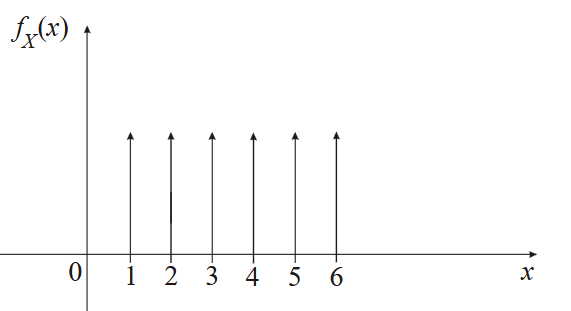
\includegraphics[scale = 0.6]{Densità di probabilità del lancio del dado.PNG}
\end{figure} 

\newpage 

Inoltre, le densità di probailità possono essere miste: 

\begin{figure}[h]
    \centering
    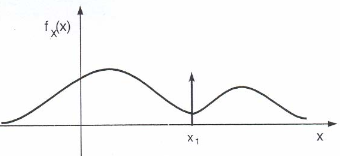
\includegraphics[scale = 0.6]{Densità di probabilità mista 1.PNG}
    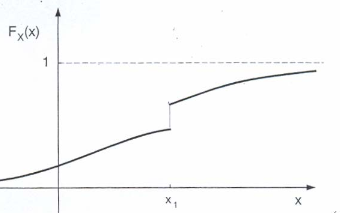
\includegraphics[scale = 0.6]{Densità di probabilità mista 2.PNG} 
\end{figure} 

Nel caso di variabile aleatoria continua, la probabilità che la X assuma un particolare valore $\overline{x}$ è uguale a zero: 

{
    \Large 
    \begin{equation}
        \Pr{\overline{x} < X \leq \overline{x} + \Delta x}
        = 
        \int_{\overline{x}}^{\overline{x} + \Delta x}
        f_X (x) dx
    \end{equation}
}


Se $\Delta x$ è molto piccolo, questa espressione può essere approssimata con: 

{
    \Large 
    \begin{equation}
        \Pr{\overline{x} < X \leq \overline{x} + \Delta x} 
        \approx 
        f_X (\overline{x}) \Delta x
    \end{equation}
}

che facendo tendere a $\Delta x$ a zero, visto che $f_X (\overline{x})$ assume necessariamente un valore finito, 
dà come risultato: 

{
    \Large 
    \begin{equation}
        \Pr{X = \overline{x}} 
        = 
        0
    \end{equation}
}

Nel caso di variabile discreta, 
la stessa conclusione vale per tutti i valori di X non ammissibili, 
mentre in corrispondenza dei valori ammissibili $x_k$ si ha: 

{
    \Large 
    \begin{equation}
        \lim_{\Delta x \rightarrow 0}
        \Pr{x_k < X \leq x_k + \Delta x}
        = 
        \Pr{X = x_k}
    \end{equation}
}

Questa formula è uguale alla foruma della densità di probabilità di una variabile discreta, quindi, tendendo $\Delta x$ a zero nel caso continuo si avrà che:

{
    \Large 
    \begin{equation}
        \Pr{x_k < X \leq x_k + \Delta x} 
        = 
        \int_{x_k}^{x_k + \Delta x} 
        \Pr{X = x_k}
        \delta (x - x_k)
        dx 
    \end{equation}
}

\newpage 

\section{Esempi di variabili aleatorie}

Si forniscono diversi tipi di esempi di variabili continue. \newline 

\subsection{Variabile uniforme} 

Densità di probabilità: 

{
    \Large 
    \begin{equation}
        f_X (x) 
        = 
        \begin{cases}
            0 
            \text{ per }
            x<a 
            \\
            \frac{1}{b - a} 
            \text{ per } 
            a \leq x \leq b 
            \\ 
            0 
            \text{ per } 
            x>b
        \end{cases}
    \end{equation}
}

\begin{figure}[h]
    \centering
    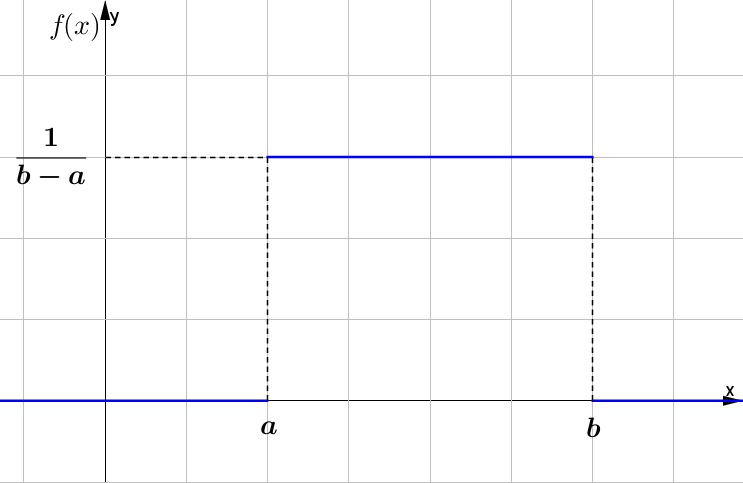
\includegraphics[scale = 0.4]{densita-distribuzione-uniforme.png}
\end{figure} 

Per integrazione, si ottiene: 

{
    \Large 
    \begin{equation}
        F_X (x) 
        = 
        \begin{cases}
            0 
            \text{ per }
            x<a 
            \\
            \frac{x-a}{b - a} 
            \text{ per } 
            a \leq x \leq b 
            \\ 
            1 
            \text{ per } 
            x>b
        \end{cases}
    \end{equation}
}

\subsection{Esponenziale unilatera} 

{
    \Large 
    \begin{equation}
        f_X (x) 
        = 
        \begin{cases} 
            0 
            \text{ per } 
            x < 0
            \\
            a \cdot \exp(-a x) 
            \text{ per } 
            x \geq 0 
        \end{cases}
    \end{equation}
} 

con $a > 0$. \newline 

Per integrazione si avrà: 

{
    \Large 
    \begin{equation}
        F_X (x) 
        = 
        \begin{cases} 
            0 
            \text{ per } 
            x < 0
            \\
            1 - \exp(-a x) 
            \text{ per } 
            x \geq 0 
        \end{cases}
    \end{equation}
} 

\subsection{Esponenziale bilatera (di Laplace)} 

Si tratta di una variabile aleatoria continua caratterizzata dalla densità di probabilità: 

{
    \Large 
    \begin{equation}
        f_X (x) 
        = 
        \frac{a}{2}
        \exp(-a \abs{x}) 
        \text{ per } 
        a > 0
    \end{equation}
}

\begin{figure}[h]
    \centering
    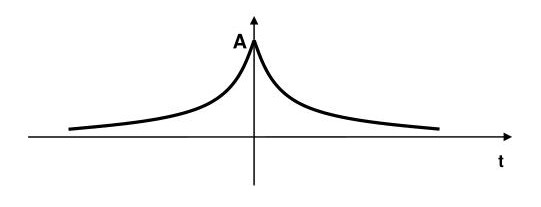
\includegraphics[scale = 0.8]{esponenziale-bilatero.jpg}
\end{figure} 

Per integrazione, si ottiene: 

{
    \Large 
    \begin{equation}
        F_X (x) = 
        \begin{cases}
            \frac{1}{2} \exp(ax) \text{ per } x<0 \\ 
            1 - \frac{1}{2} \exp(-ax) \text{ per } x \geq 0 
        \end{cases}
    \end{equation}
}

\subsection{Gaussiana} 

Si tratta di una variabile aleatoria continua caratterizzata dalla densità di probabilità: 

{
    \Large 
    \begin{equation}
        f_X (x) 
        = 
        \frac{1}{\sqrt{2 \pi} \sigma} 
        \exp[- \frac{(x - \mu)^{2}}{2 \sigma ^{2}}]
    \end{equation}
}

Alcune considerazioni riguardo alla formula della gaussiana. \newline 

$f_X (x)$ assume il valore massimo in $x = \mu$. \newline 

$(x- \mu)^{2}$ è una relazione quadratica, quindi è una relazione non lineare. \newline 

$\sigma$ più è piccola, più è stretta la gaussiana. \newline 

Esempi di gaussiane con valori differenti: 

\begin{figure}[h]
    \centering
    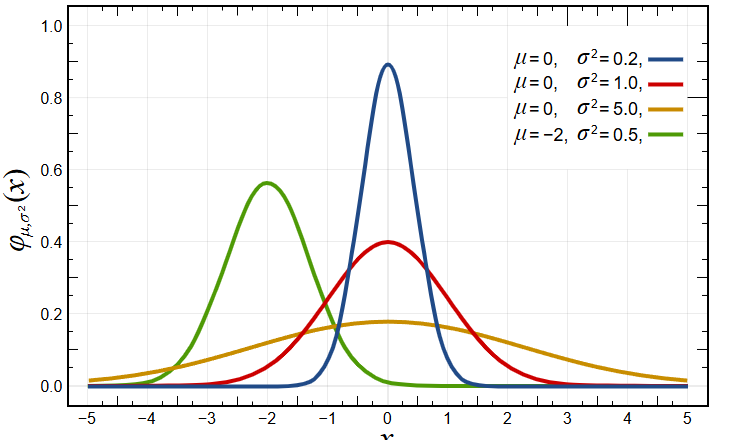
\includegraphics[scale = 0.6]{Gaussiana normalizzata.PNG}
\end{figure} 

Adesso proporemo a riscrivere $F_X (x)$ con una relazione "pseudo-lineare". \newline 

Introducendo il cambiamento di variabile: 

{
    \Large 
    \begin{equation}
        y = \frac{\xi - \mu}{\sqrt{2} \sigma} 
        \rightarrow 
        d\xi = \sqrt{2} \sigma dy
    \end{equation}
}

Grazie a questa sostituzione, possiamo avere $F_X (x)$ come: 

{
    \Large 
    \begin{equation}
        F_X (x) 
        = 
        \frac{1}{\sqrt{\pi}} 
        \int_{-\infty}^{\frac{x - \mu}{\sqrt{2} \sigma}} 
        \exp(-y^{2}) dy
    \end{equation}
} 

Si consideri ora la seguente definizione di $erfc(x)$ (funzione errore complementare): 

{
    \Large 
    \begin{equation}
        erfc(x) 
        = 
        \frac{2}{\sqrt{\pi}} 
        \int_{x}^{\infty} 
        \exp(- y^{2}) dy
    \end{equation}
}

Tale funzione verifica le seguenti proprietà: 

{
    \Large 
    \begin{equation}
        \begin{cases}
            erfc(-\infty) = 2 \\ 
            erfc(0) = 1
        \end{cases}
    \end{equation}
}

Non è una densità di probabilità perchè la funzione a $-\infty \neq 1$. \newline 

Si può anche considerare la funzione $\erf(x)$ (funzione errore), così definita:

{
    \Large 
    \begin{equation}
        \begin{split}
            \erf(x) 
            &= 
            1 - erfc(x) 
            \\ 
            &= 
            \frac{2}{\sqrt{\pi}}
            \int_{0}^{+ \infty} 
            \exp(- y^{2}) dy 
            - 
            \frac{2}{\sqrt{\pi}}
            \int_{x}^{+ \infty} 
            \exp(- y^{2}) dy
            \\ 
            &= 
            \frac{2}{\sqrt{\pi}}
            \int_{0}^{x} 
            \exp(- y^{2}) dy  
        \end{split}
    \end{equation}
}


Utilizzando le funzioni $erfc(x)$ e $\erf(x)$, possiamo riscrivere $F_X (x)$ come: 

{
    \Large 
    \begin{equation}
        \begin{split}
            F_X (x) 
            &= 
            \frac{1}{\sqrt{\pi}}
            \int_{- \infty}^{\frac{x - \mu}{\sqrt{2} \sigma}} 
            \exp(-y^{2}) dy
            \\ 
            &= 
            \frac{1}{\sqrt{\pi}}
            \int_{- \infty}^{ + \infty} 
            \exp(-y^{2}) dy 
            - 
            \frac{1}{\sqrt{\pi}}
            \int_{\frac{x - \mu}{\sqrt{2} \sigma}}^{ + \infty} 
            \exp(-y^{2}) dy
            \\ 
            &=
            1 - \frac{1}{2} erfc(\frac{x - \mu}{\sqrt{2} \sigma})
            \\ 
            &= 
            1 - \frac{1}{2} 
            [1 - \erf(\frac{x - \mu}{\sqrt{2} \sigma})]
            \\ 
            &= 
            \frac{1}{2} 
            [1 + \erf(\frac{x - \mu}{\sqrt{2} \sigma})]
        \end{split}
    \end{equation}
}


Generalmente si prendere il valore di $erfc(\frac{x - \mu}{\sqrt{2} \sigma})$ da una tabella e 
si sostituisce alla formula $ 1 - \frac{1}{2} erfc(\frac{x - \mu}{\sqrt{2} \sigma})$. \newline 


Inoltre, possiamo scrivere la seguente relazione: 

{
    \Large 
    \begin{equation}
        \begin{split}
            erfc(-x) 
            &=
            \frac{2}{\sqrt{\pi}}
            \int_{-x}^{\infty}
            \exp(-y^{2}) dy
            \\ 
            &=
            \frac{2}{\sqrt{\pi}}
            \int_{-x}^{0}
            \exp(-y^{2}) dy 
            + 
            \frac{2}{\sqrt{\pi}}
            \int_{0}^{+ \infty}
            \exp(-y^{2}) dy  
            \\ 
            &= 
            \frac{2}{\sqrt{\pi}}
            \int_{0}^{x}
            \exp(-y^{2}) dy
            + 
            1 
            \\ 
            &=
            1 + \erf(x)    
        \end{split}
    \end{equation}
}

invece: 

{
    \Large 
    \begin{equation}
        \begin{split}
            \erf(-x) 
            &= 
            \frac{2}{\sqrt{\pi}} 
            \int_{0}^{-x} 
            \exp(- y^{2}) dy
            \\ 
            &= 
            -\frac{2}{\sqrt{\pi}} 
            \int_{0}^{x} 
            \exp(- y^{2}) dy 
            \\ 
            &=
            - \erf(x)
        \end{split}
    \end{equation}
}

Da questa ultima equazione, notiamo che la funzione $\erf(x)$ è una funzione dispari. \newline 

Altra funzione erfc(x) che si considera la funzione Q(x) così definita: 

{
    \Large 
    \begin{equation}
        Q(x) = \frac{1}{\sqrt{2 \pi}} 
        \int_{x}^{\infty}
        \exp(- \frac{y^{2}}{2}) 
        dy
    \end{equation}
}

Con un semplice cambiamento di variabile $(t = \frac{y}{\sqrt{2}})$, possiamo riscrivere Q(x) come: 

{
    \Large 
    \begin{equation}
        Q (x) = \frac{1}{2} erfc(\frac{x}{\sqrt{2}})
    \end{equation}
} 


\subsection{Rayleigh} 

Si tratta di una variabile aleatoria continua caratterizzata dalla densità di probabilità: 

{
    \Large 
    \begin{equation}
        f_X (x) 
        = 
        \begin{cases}
            0 \text{ per } x < 0 \\
            \frac{x}{\sigma ^{2}} \exp(- \frac{x^{2}}{2 \sigma ^{2}}) \text{ per } x \geq 0
        \end{cases}
    \end{equation}
}

Per integrazione si ottiene: 

{
    \Large 
    \begin{equation}
        F_X (x) = 
        \begin{cases}
            0 \text{ per } x < 0 \\ 
            1 - \exp (- \frac{x^{2}}{2 \sigma^{2}}) \text{ per } x \geq 0
        \end{cases}
    \end{equation}
}

\subsection{Binomiale} 

Si tratta di una variabile aleatoria discreta associata all'esperimento di Bernoulli: 

{
    \Large 
    \begin{equation}
        f_X (x) 
        = 
        \sum_{k = 0}^{n}
        \binom{n}{k}
        p^{k}
        (1 - p)^{n - k}
        \delta(x - k)
    \end{equation}
}

dove $X = k$ comporta che, in n prove ripetute, per k volte si è avuto l'esito che ha la probabilità p di verificarsi. \newline 

Possiamo variare p. \newline 

Ponendo ad esempio $p=\frac{1}{2}$, $f_X (x)$ diventa: 

{
    \Large 
    \begin{equation}
        f_X (x) 
        = 
        \sum_{k = 0}^{n}
        \binom{n}{k}
        \frac{1}{2^{n}}
        \delta(x - k)
    \end{equation}
}

Per integrazione, $F_X (x)$ sarà: 

{
    \Large 
    \begin{equation}
        F_X (x) 
        = 
        \frac{1}{2^{n}}
        \sum_{k=0}^{n}
        \binom{n}{k}
        u(x - k)
    \end{equation}
}

\subsection{Poisson} 

Si tratta di una variabile aleatoria discreta caratterizzata dalla densità di probabilità: 

{
    \Large 
    \begin{equation}
        \sum_{k = 0}^{+ \infty}
        \frac{\lambda ^{k}}{k !}
        \exp(- \lambda)
        \delta(x-k)
    \end{equation}
}

Per integrazione: 

{
    \Large 
    \begin{equation}
        F_X (x) = \exp(-\lambda) \sum_{k = 0}^{+ \infty}
        \frac{\lambda^{k}}{k !} 
        u(x - k)
    \end{equation}
}

\newpage

\section{Indicatori statistici} 

La conoscenza della funzione densità di probabilità (il che è lo stesso, della distribuzione di probabilità cumulativa) 
fornisce una descrizione completa del comportamento di una variabile aletoria. \newline 

In molti casi, una conoscenza così dettagliata non è necessaria e ci si può accontentare della determinazione di alcuni parametri caratteristici, 
i quali verranno indicati di seguito. \newline 

\subsection{Valore medio}

Per una variabile aleatoria X con densità di probabilità $f_X (x)$, il valore è fornito dale seguente integrale: 

{
    \Large 
    \begin{equation}
        m_X = \int_{- \infty}^{\infty} x f_X (x) dx
    \end{equation}
}

In alcuni casi, si indica il valore medio con la lettera, con la lettera E (dall'inglese Expectation), oppure con le parentesi $< >$: 

{
    \Large 
    \begin{equation}
        <X> = E\{X\} = m_X
    \end{equation}
}

Il valore medio ha, essenzialmente, il significato di "baricentro" attorno al quale si distribuiscono i valori della variabile aleatoria. \newline 

Non sempre $m_X$ coincide ad un valore possibile (si pensi ad esempio al $m_x$ di un lancio del dado). \newline 

Se la variabile aleatoria è discreta, $m_X$ si può scrivere come: 

{
    \Large 
    \begin{equation}
        \begin{split}
            m_X 
            &= 
            \int_{-\infty}^{+\infty}
            x f_X (x) dx 
            \\ 
            &= 
            \int_{-\infty}^{+\infty}
            x \sum_{k} p_k \delta(x - x_k) dx
            \\  
            &= 
            \sum_{k} p_k 
            \int_{-\infty}^{+\infty}
            x \delta(x - x_k) dx 
            \\ 
            &= 
            \sum_{k}
            p_k x_k
        \end{split}
    \end{equation}
}

Inoltre, nell'ultimo passaggio, si è sfruttato la proprietà di campionamento della Delta di Dirac. \newline 

Per semplificare la notazione: 

{
    \Large 
    \begin{equation}
        \Pr{X = x_k} = p_k
    \end{equation}
}

Per una funzione generale: 

{
    \Large 
    \begin{equation}
        Y = g(X)
    \end{equation}
} 

si può calcolare il valore della variabile media:

{
    \Large 
    \begin{equation}
        m_Y 
        = 
        \int_{- \infty}^{+ \infty} 
        g(x) f_X (x) dx 
    \end{equation}
}

Inoltre, si può calcolare la funzione di densità di probabilità di $f_Y (y)$ 
a partire dalla conoscenza della $f_X (x)$. \newline 

$m_Y$ si può calcolare come: 

{
    \Large 
    \begin{equation}
        m_Y 
        = 
        \int_{-\infty}^{+ \infty}
        y f_Y (y) dy
    \end{equation}
}


La conoscenza di $f_Y (y)$ non è strettamente necesaria perchè spesso si utlizza la formula 
di $m_y$ usando $f_X$. \newline 

\subsection{Valore quadratico medio} 

Si tratta di una particolare applicazione della $m_y = \int_{-\infty}^{+\infty} g(x) f_X (x) dx$ in cui: 

{
    \Large 
    \begin{equation}
        Y = g(X) = X^{2}
    \end{equation}
}

quindi possiamo scrivere che il valore quadratico medio $<X^{2}>$ come:

{
    \Large 
    \begin{equation}
        <X^{2}> = \int_{-\infty}^{+ \infty} x^{2} f_X (x) dx
    \end{equation}
}

Per una variabile discreta, il valore quadratico medio è: 

{
    \Large 
    \begin{equation}
        \begin{split}
            <X^{2}> 
            &= 
            \int_{-\infty}^{+\infty}
            x^{2} f_X (x) dx 
            \\ 
            &= 
            \int_{-\infty}^{+\infty}
            x^{2} 
            \sum_{k} 
            p_k 
            \delta(x - x_k)
            dx 
            \\ 
            &= 
            \sum_{k} 
            p_k
            \int_{-\infty}^{+\infty}
            x^{2}  
            \delta(x - x_k)
            dx
            \\ 
            &= 
            \sum_{k}
            p_k 
            x_k ^{2}
        \end{split}
    \end{equation}
}

\subsection{Varianza} 

Per una variabile aleatoria X con densità di probabilità $f_X (x)$, 
la varianza è fornita dal seguente integrale: 

{
    \Large 
    \begin{equation}
        \begin{split}
            \sigma_X ^{2}    
            &= 
            <(X - m_X) ^{2} >
            \\ 
            &= 
            \int_{-\infty}^{+\infty}
            (x - m_X) ^{2}
            f_X (x) dx 
        \end{split}
    \end{equation}
}

La varianza misura il livello di dispersione della variabile aleatoria intorno al valore medio. \newline 

La sua radice quadrata $\sigma$ prende il nome di deviazione standard (o scarto quadratico medio). \newline 

Inoltre, la relazione tra varianza, valore quadratico medio e valore medio è la segeunte: 

{
    \Large 
    \begin{equation}
        \begin{split}
            \sigma_X ^{2}
            &= 
            \int_{- \infty}^{ + \infty}
            (x - m_x)^{2} f_X (x) dx 
            \\ 
            &= 
            \int_{- \infty}^{ + \infty}
            x^{2} f_X (x) dx  
            - 2 m_X 
            \int_{- \infty}^{ + \infty}
            x f_X (x) dx
            + m_X ^{2} 
            \int_{- \infty}^{ + \infty}
            f_X (x) dx 
            \\ 
            &= 
            \int_{- \infty}^{ + \infty}
            x^{2} f_X (x) dx  
            - 2 m_X 
            \cdot m_X
            + m_X ^{2} 
            \cdot 1 
            \\ 
            &=
            <X^{2}> - 2 m_X ^{2} + m_X ^{2}
            \\ 
            &= 
            <X^{2}> -  m_X ^{2}
        \end{split}
    \end{equation}
} 

avendo sfruttato, nell'ultimo termine, anche la proprietà di normalizzazione. \newline 

\subsection{Momenti e momenti centrali}

Data una variabile aleatoria X con densità di probabilità $f_X (x)$, si definisce 
momento di ordine j di tale variabile il seguente integrale: 

{
    \Large 
    \begin{equation}
        \begin{split}
            M_j 
            &= 
            <X ^{j}> 
            \\
            &= 
            \int_{- \infty}^{+ \infty} 
            x^{j} f_X (x) dx 
            \text{ per }
            j = 1, 2, 3, ...
        \end{split}
    \end{equation}
}

Per $j=1$, si ha il valore medio, per $j=2$ si ha il valore quadratico medio. \newline 

Per la stessa variabile aleatoria X, si definisce momento centrale di ordine j il seguente integrale: 

{
    \Large 
    \begin{equation}
        \begin{split}
            \sigma_j 
            &= 
            <(X - m_X) ^{j}> 
            \\ 
            &=
            \int_{ - \infty}^{+ \infty} 
            (x - m_x)^{j} f_X (x) dx 
            \\ 
            &= 
            \int_{ - \infty}^{+ \infty} 
            (x - M_1)^{j} f_X (x) dx 
            \text{ per } 
            j = 2, 3, ...
        \end{split}
    \end{equation}
}

per $j = 2$, si riottiene la varianza; 
si ha dunque 
$\sigma_2 = \sigma_X ^{2}$. \newline 

Oppure, sviluppando la potenza j-esima, possiamo scrivere $\sigma_j$ come: 

{
    \Large 
    \begin{equation}
        \sigma_j 
        = 
        \sum_{k = 0}^{j} 
        \binom{j}{k} 
        (-M_1) ^{k} 
        M_{j -k} 
        \text{ per }
        j = 2, 3, ...
    \end{equation}
}

I momenti di una variabile aleatoria, 
oltre alle espressioni integrali precedentemente scritte, possono essere ricavati con 
la funzione caratteristica così definita: 

{
    \Large 
    \begin{equation}
        \begin{split}
            C_X (u) 
            &= 
            <\exp(\jmath u x)>    
            \\ 
            &= 
            \int_{- \infty}^{+ \infty} 
            \exp(\jmath u x) 
            f_X (x) dx
        \end{split}
    \end{equation}
}

La formula appena scritta è simile alla formula della trasformata di Fourier, 
al posto della t c'è la variabile u, e al posto di $\omega$ c'è la varibile x. \newline

Come la trasformata di Fourier, possiamo definire la sua anti-trasformata, quindi dai momenti j-esimi 
si può ricavare $f_X (x)$ come: 

{
    \Large 
    \begin{equation}
        f_X (x)
        = 
        \frac{1}{2\pi}
        \int_{-\infty}^{+ \infty} 
        \exp(- \jmath u x) C_X (u) du
    \end{equation}
} 

Grazie a questo legame e alla funzione caratteristica, possiamo scrivere questa relazione: 

{
    \Large 
    \begin{equation}
        M_j = (-\jmath)^{j} \left. \frac{d^{j} C(u)}{du^{j}} \right|_{u = 0} 
        \text{ per } j = 1, 2, ...
    \end{equation}
}

Inoltre, grazie a questa relazione, possiamo anche scrivere la seguente relazione: 

{
    \Large 
    \begin{equation}
        \begin{split}
            (-\jmath)^{j} \left. \frac{d^{j} C(u)}{du^{j}} \right|{u = 0} 
            &= 
            (-\jmath) ^{j} \frac{d^{j}}{du^{j}}
            \left. 
            \int_{-\infty}^{+ \infty}
            \exp(\jmath u x)
            f_X (x) dx
            \right|_{u = 0}
            \\ 
            &=  
            (-\jmath) ^{j} 
            \left. 
            \int_{-\infty}^{+ \infty}
            \frac{d^{j}}{du^{j}}
            \exp(\jmath u x)
            f_X (x) dx
            \right|_{u = 0} 
            \\
            &= 
            (-\jmath) ^{j} 
            (\jmath) ^{j}
            \left. 
            \int_{-\infty}^{+ \infty}
            x^{j}
            \exp(\jmath u x)
            f_X (x) dx
            \right|_{u = 0}
            \\ 
            &=
            \int_{- \infty}^{+ \infty}
            x^{j} 
            f_X (x) dx 
            \\ 
            &= 
            M_j 
        \end{split}
    \end{equation}
}


Per una variabile aleatoria discreta, la funzione caratteristica, ponendo
{
    \Large 
    \begin{equation}
     \Pr{X = x_k} = p_k   
    \end{equation}
}  

diventa: 

{
    \Large 
    \begin{equation}
        C_X (u) = \sum_{k} p_k \exp(\jmath u x_k)
    \end{equation}
}

\newpage 

\section{Funzioni di variabile aleatoria}

In molti problemi di interesse pratico, nota che sia la descrizione statistica di una variabile 
aleatoria X, per esempio, tramite la conoscenza della densità di probabilità $f_X(x)$ si è interessati 
a risalire alla descrizione statistica di una variabile aleatoria Y legata a X dalla relazione: 

{
    \Large 
    \begin{equation}
        Y = g(X)
    \end{equation}
}

Se g(X) è una funzione monotona, crescente o decrescente, il problema può essere immediatamente risolto; 
si verifica infatti che risulta: 

{
    \Large 
    \begin{equation}
        f_Y (y) 
        = 
        \left. 
            \frac{f_X (x)}{\abs{g^{'} (x)}}
        \right|_{x = g^{-1} (y)} 
    \end{equation}
}

dove si è posto: 

{
    \Large 
    \begin{equation}
        g^{'} (x) = \frac{d g(x)}{dx}
    \end{equation}
} 

e $g^{-1} (Y)$ la funzione inversa di $ Y = g(X)$ (che esiste sicuramente perchè la funzione è monotona). \newline 

L'equazione di $f_Y (y)$ sarà presa senza dimostrazione. \newline 

Nel caso in cui la funzione $g(x)$ non sia monotona, 
ma l'intervallo di variabilità della X decomponibile in un numero finito di regioni in cui la funzione è monotona, 
la densità di probabilità della variabile aleatoria Y può essere ricavata come: 

{
    \Large 
    \begin{equation}
        f_Y (y) 
        = 
        \sum_{i} 
        \left.
        \frac{f_X (x_i)}{\abs{g^{'} (x_i)}} 
        \right|_{x_i = g^{-1} (y)}
    \end{equation}
}

dove l'insieme $\{x_i\}$ è costituito da tutte le soluzione dell'equazione $g(x)$. \newline 

Esplicitamente, ciò equivale a dire che: 

\begin{itemize}
    \item si individuano i sottointervalli della variabile aleatoria X in cui g(x) è monotona 
    \item si determinano i corrispondenti intervalli della variabile aleatoria Y 
    \item entro ciascun intervallo si applica la formula di $ f_Y (y) 
    = 
    \left. 
        \frac{f_X (x)}{\abs{g^{'} (x)}}
    \right|_{x = g^{-1} (y)}$, che fornirà l'andamento "locale" della densità di probabilità cercata 

    \item si sovrappongono i risultati parziali così ottenuti


\end{itemize}

\newpage 

\section{Coppie di variabili aleatorie}

Consideriamo una coppia di variabili aleatorie X e Y. \newline 

Singolarmente, esse saranno caratterizzate dalle rispettive densità di probabilità $f_X (x)$ e $f_Y (y)$ 
o, il che è lo stesso delle rispettive densità di probabilità cumulativa $F_X (x)$ e $F_Y (y)$. \newline 

Ciò che però può essere di interesse è la descrizione statistica congiunta di queste variabili. \newline 

Possiamo definire la distribuzione di probabilità congiunta delle due variabili la seguente funzione: 

{
    \Large 
    \begin{equation}
        F_{XY} (x, y) = \Pr{X \leq x, Y \leq y}
    \end{equation}
}

La valutazione della distribuzione di probabilità congiunta risulta particolarmente semplice nel caso in cui le variabile X e Y sono tra loro statisticamente indipendenti. \newline 


Grazie alla proprietà di indipendenza, possiamo scrivere: 

{
    \Large 
    \begin{equation}
        \begin{split}
            F_{XY} 
            &= 
            \Pr{X \leq x} \cdot \Pr{Y \leq y} 
            \\
            &= 
            F_X (x) \cdot F_Y (y) 
        \end{split}
    \end{equation}
}

Come nel caso nelle funzioni ad una variabile, per $F_{XY} (x, y)$ possiamo determinare 
le properità statistiche marginali: 

\begin{enumerate}
    \item $F_{XY} (x, y)$ assume valori appartenenti all'intervallo $[0 , 1]$, cioè: 
        {
            \Large 
            \begin{equation}
                0 \leq F_{XY} (x, y) \leq 1
            \end{equation}
        }

    \item  $F_{XY} (x, y_0)$ (si legge il valore di $y_0$ della variabile Y) è monotona non decrescente nella variabile X e continua da destra in questa variabile; \\ 
       analogamente $F_{XY} (x_0, y) $, come si scelga il valore $x_0$ della variabile X, è monotona non decrescente nella variabile Y e continua da destra in questa variabile 

    \item $F_{XY} (x, y)$ soddisfa le segeunti uguaglianze: 
    
            {
                \Large 
                \begin{equation}
                    \begin{split}
                        F_{XY} (-\infty, y)
                        &= 
                        \Pr{X \leq - \infty, Y \leq y}
                        \\ 
                        &= 
                        0
                    \end{split}
                \end{equation}
            }

            {
                \Large 
                \begin{equation}
                    \begin{split}
                        F_{XY} (x , -\infty)
                        &= 
                        \Pr{X \leq x, Y \leq -\infty}
                        \\ 
                        &= 
                        0
                    \end{split}
                \end{equation}
            } 

            {
                \Large 
                \begin{equation}
                    \begin{split}
                        F_{XY} (-\infty, - \infty)
                        &= 
                        \Pr{X \leq - \infty, Y \leq -\infty}
                        \\ 
                        &= 
                        0
                    \end{split}
                \end{equation}
            }

    \item le distribuzioni di probabilità cumulative delle variabili X e Y (distribuzioni marginali) si ottengono come segue: 
                {
                    \Large 
                    \begin{equation}
                        F_X (x) = F_{XY} (x, + \infty) 
                        \text{ saturazione della variabile y}
                    \end{equation}
                } 

                {
                    \Large 
                    \begin{equation}
                        F_Y (y) = F_{XY} (+ \infty, y) 
                        \text{ saturazione della variabile x}
                    \end{equation}
                }
    
    \item il limite di $F_{XY} (x, y)$ quando sia x che y tendono a $+ \infty$ è unitario, si ha cioè:
                {
                    \Large 
                    \begin{equation}
                        F_{XY} (+ \infty, + \infty) = 1 
                        \text{ evento certo}
                    \end{equation}
                }
    \item la probabilità dell'evento "rettangolare" :$\{x_1 < X \leq x_2, y_1 < Y \leq y_2\}$ può essere calcolato mediante la relazione seguente: 
                {
                    \Large 
                    \begin{equation} 
                        \begin{split}
                            \Pr{x_1 < X \leq x_2, y_1 < Y \leq y_2}
                            &= 
                            F_{XY} (x_2, y_2) 
                            \\
                            &- F_{XY} (x_1, y_2)
                            \\
                            &-F_{XY} (x_2, y_1) 
                            \\
                            &+ F_{XY} (x_1, y_1)    
                        \end{split}
                    \end{equation}
                }
    
\end{enumerate}

\begin{figure}[h]
    \centering
    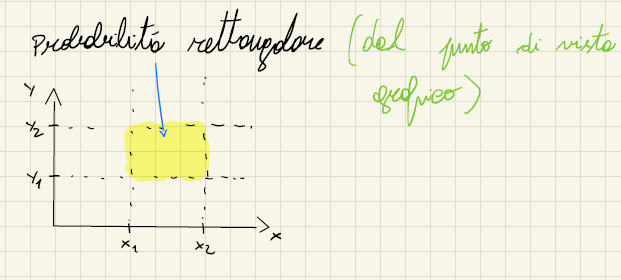
\includegraphics[scale = 0.8]{Densità di probabilità congiunta graficamente.PNG}
\end{figure} 


Quanto scritto sin qui per le distribuzioni di probabilità cumulativa può essere esteso alla densità di probabilità. \newline 

Definiamo allora la seguente densità di probabilità congiunta: 

{
    \Large 
    \begin{equation}
        f_{XY} (x, y) 
        = 
        \frac{\partial ^{2} F_{XY} (x, y)}{\partial x \partial y}
    \end{equation}
}

Possiamo calcolarci la funzione inversa per calcolarci la distribuzione di probabilità congiunta a partire dalla densità di probab: 

{
    \Large 
    \begin{equation}
        F_{XY} (x, y) 
        =
        \int_{\alpha = -\infty}^{x}
        \int_{\beta = -\infty}^{y}
        f_{XY} (\alpha, \beta) 
        d\alpha d\beta 
    \end{equation}
}

Se le variabili sono statisticamente indipendenti, si ha: 

{
    \Large 
    \begin{equation}
        f_{XY} (x, y)
        = 
        f_{X} (x)
        \cdot
        f_{Y} (y)
    \end{equation}
}

Come la distribuzione di probabilità cumulativa, anche la densità di probabilità congiunta gode di una serie di probabilità 
gode di una serie di proprietà; le più importanti sono le seguenti: 

\begin{enumerate}
    \item $f_{XY} (x, y)$ assume valori non negativi, cioè: 
    {
        \Large 
        \begin{equation}
            f_{XY} (x, y) \geq 0
        \end{equation}
    }

    \item l'integrale di $f_{XY}$ sull'intero piano x-y vale 1 (proprietà di normalizzazione), cioè: 
    {
        \Large 
        \begin{equation}
            \int_{x = -\infty}^{+ \infty}
            \int_{y = -\infty}^{+ \infty}
            f_{XY} (x, y) dx dy = 1
        \end{equation}
    }

    \item le densità di probabilità marginali delle variabili X e Y si ottengono come segue:
    {
        \Large 
        \begin{equation}
            f_X (x) = \int_{-\infty}^{\infty} f_{XY} (x, y) dy 
        \end{equation}
    }
    Facendo l'integrale su dy, si satura y 

    {
        \Large 
        \begin{equation}
            f_Y (y) = \int_{-\infty}^{\infty} f_{XY} (x, y) dx 
        \end{equation}
    }
    Facendo l'integrale su dy, si satura x 
    
    \item la probabilità di un evento $A = \{(X, Y) \in D \}$ individuato da un dominio D nel piano x-y, è data da: 
    
    {
        \Large 
        \begin{equation}
            \Pr(A) = \iint \limits_{D} f_{XY} (x, y) \,dx \,dy
        \end{equation}
    }
    
\end{enumerate}

\newpage 

\section{Densità di probabilità condizionata} 

Date due variabili aleatorie X e Y, si può introdurre la densità di probabilità condizionata della variabile aleatoria Y, rispetto all'evento $\{X = x\}$: 

{
    \Large 
    \begin{equation}
        f_{Y | X} (y | x)
        = 
        \frac{f_{XY} (x, y)}{f_X (x)}
    \end{equation}
}

Dall'altro canto, per definizione: 

{
    \Large 
    \begin{equation}
        f_{Y | X} (y | x)
        = 
        \frac{d F_{Y|X} (y | x)}{dy}
    \end{equation}
}


e quindi, la distribuzione di probabilità condizionata della variabile aleatoria Y, rispetto all'evento $\{ X = x\}$ risutla: 

{
    \Large 
    \begin{equation}
        \begin{split}
            F_{Y | X} (y | x) 
            &= 
            \int_{\beta = -\infty}^{y}
            f_{Y | X} (\beta | x) d\beta 
            \\ 
            &= 
            \int_{\beta = -\infty}^{y}
            \frac{f_{XY} (x, \beta)}{f_X (x)} 
            d\beta 
            \\ 
            &=
            \frac{ 
            \int_{\beta = -\infty}^{y}
            f_{XY} (x, \beta)} 
            {f_X (x)} 
            d\beta
        \end{split}
    \end{equation}
}

Scambiando i ruoli X e Y, relazioni analoghe si trovano per la densità di probabiltà condizionata della variabile aleatoria X, rispetto all'evento $\{ Y = y\}$. \newline 

Nel caso di variabili aleatorie X e Y statisticamente indipendenti:

{
    \Large 
    \begin{equation}
        f_{Y | X} (y | x) = f_Y (y)
    \end{equation}
}

e 

{
    \Large 
    \begin{equation}
        f_{X | Y} (x | y) = f_X (x)
    \end{equation}
}

Nel caso generale, quando X e Y possono essere anche non statisticamente indipendenti: 

{
    \Large 
    \begin{equation}
        f_{X | Y} (x | y) f_Y (y)
        = 
        f_{Y | X} (y | x) f_X (x)
    \end{equation}
}

che a sua volta richiama la formula di Bayes. \newline 

\newpage

\section{Momenti congiunti e momenti centrali congiunti} 

Utilizzando le funzioni $F_{XY} (x, y)$ e $f_{XY} (x, y)$, le definizioni di momenti e momenti centrali fornite in precedenza per una variabile 
aleatoria possono essere estese a coppie di variabili aleatorie. \newline 

Si definisce un momento congiunto di ordine (j, k) della coppia di variabili aleatorie X e Y il seguente integrale: 
{
    \Large 
    \begin{equation}
        \begin{split}
            M_{j k} 
            &= 
            <X^{j} Y^{k}>
            \\ 
            &= 
            \int_{x = -\infty}^{+ \infty}
            \int_{y = -\infty}^{+ \infty}
            x^{j} y^{k} 
            f_{XY} (x, y) 
            dx 
            dy 
            \text{ per } 
            j,k = 0, 1, 2, 3, ...
        \end{split}
    \end{equation}
} 

Particolarmente importante è il momento congiunto di ordine (1, 1), il quale risulta: 

{
    \Large 
    \begin{equation}
        \begin{split}
            M_{1 1} 
            &= 
            <X Y>
            \\ 
            &= 
            \int_{x = -\infty}^{+ \infty}
            \int_{y = -\infty}^{+ \infty}
            x y 
            f_{XY} (x, y) 
            dx 
            dy 
        \end{split}
    \end{equation}
}

Il momento congiunto di ordine (1, 1) prende il nome di correlazione. \newline 

Nel caso di variabili statisticamente indipendenti, avremo che: 

{
    \Large 
    \begin{equation}
        \begin{split}
            M_{1 1} 
            &= 
            <X Y>
            \\ 
            &= 
            \int_{x = -\infty}^{+ \infty}
            \int_{y = -\infty}^{+ \infty}
            x y 
            f_{X} (x) 
            f_{Y} (y) 
            dx 
            dy 
            \\ 
            &= 
            \int_{x = -\infty}^{+ \infty}
            x  
            f_{X} (x)
            dx 
            \int_{y = -\infty}^{+ \infty}
            y 
            f_{Y} (y) 
            dy 
            \\ 
            &= 
            m_X m_Y
        \end{split}
    \end{equation}
}

Se $ M_{1 1} =  m_X m_Y $ è verificata, si dice che le variabili X e Y sono tra loro incorrelate. \newline 

È certamente vero che la statistica indipendenza implica l'incorrelazione, non è detto il contrario. \newline 

Un caso particolare si verifica quando le variabili sono incorrelate e una di esse ha valor medio nullo; 
in questo caso: 

{
    \Large 
    \begin{equation}
        \begin{split}
            M_{1 1}
            &= 
            m_X m_Y 
            \\
            &= 
            0     
        \end{split}
    \end{equation}
}

Per estensione della terminologia introdotta nela teoria dei segnali determinati, si dice che le variabili 
X e Y, che verificano la condizione $M_{1 1} = 0$, sono tra loro ortogonali. \newline 

Quindi, l'ortogonalità può essere verificata anche se le variabili non sono incorrelate. \newline 

Dalla definizione di momento congiunto di ordine (j, k), possiamo avere: 

{
    \Large 
    \begin{equation}
        M_{1 0} = <X> = m_X
    \end{equation}
}

{
    \Large 
    \begin{equation}
        M_{0 1} = <Y> = m_Y
    \end{equation}
}

Si definisce momento centrale congiunto di ordine (j, k) il seguente integrale:

{
    \Large 
    \begin{equation}
        \begin{split}
            \sigma_{jk}
            &= 
            <(X - m_x)^{j} (Y - m_Y)^{j} >
            \\
            &= 
            \int_{x = -\infty}^{+ \infty}
            \int_{y = -\infty}^{+ \infty}
            (x - m_X)^{j}
            (y - m_Y)^{k} 
            f_{XY} (x, y) 
            dx dy 
            \\
            &\text{ per }
            j, k = 1, 2, ...
        \end{split}
    \end{equation}
}


Anche qui riveste particolare importanza il caso $j=k=1$: 

{
    \Large 
    \begin{equation}
        \begin{split}
            \sigma_{11}
            &= 
            <(X - m_x) (Y - m_Y) >
            \\
            &= 
            \int_{x = -\infty}^{+ \infty}
            \int_{y = -\infty}^{+ \infty}
            (x - m_X)
            (y - m_Y) 
            f_{XY} (x, y) 
            dx dy 
        \end{split}
    \end{equation}
}

$\sigma_{11}$ prende il nome di covarianza. \newline 

La covarianza, può essere espressa in funzione dei momenti definiti precedentemente: 

{
    \Large 
    \begin{equation}
        \begin{split}
            \sigma_{11}
            &= 
            <(X - m_x) (Y - m_Y) >
            \\
            &= 
            \int_{x = -\infty}^{+ \infty}
            \int_{y = -\infty}^{+ \infty}
            (x - m_X)
            (y - m_Y) 
            f_{XY} (x, y) 
            dx dy
            \\  
            &=
            \int_{x = -\infty}^{+ \infty}
            \int_{y = -\infty}^{+ \infty}
            x
            y  
            f_{XY} (x, y) 
            dx dy
            \\
            &-m_X
            \int_{x = -\infty}^{+ \infty}
            \int_{y = -\infty}^{+ \infty}
            y  
            f_{XY} (x, y) 
            dx dy 
            \\
            &-m_Y
            \int_{x = -\infty}^{+ \infty}
            \int_{y = -\infty}^{+ \infty}
            x  
            f_{XY} (x, y) 
            dx dy
            \\
            &+m_Xm_Y
            \int_{x = -\infty}^{+ \infty}
            \int_{y = -\infty}^{+ \infty}
            f_{XY} (x, y) 
            dx dy 
            \\
            &= 
            M_{11} -m_X m_Y -m_Y m_X + m_X m_Y \cdot 1 
            \\
            &= 
            M_{11} -m_X m_Y m_X m_Y + m_X m_Y
            \\ 
            &= 
            M_{11} -m_X m_Y
        \end{split}
    \end{equation}
}

Se le variabili sono incorrelate (e lo sono certamente quando sono statisticamente indipendenti), 
è chiaro che risulta: 

{
    \Large 
    \begin{equation}
        \sigma_{11} = 0
    \end{equation}
}

Proprio in virtù di questo risultato, si conviene assumere $\sigma_{11}$ come misura della correlazione statistica di due variabili aleatorie. \newline 

Generalmente, $\sigma_{11}$ viene normalizzato e usa scegliere questo rapporto: 

{
    \Large 
    \begin{equation}
        \begin{split}
            \rho_{XY}
            &= 
            \frac{\sigma_{11}}{\sigma_X \sigma_Y}
            \\
            &= 
            \frac{\sigma_{11}}{\sqrt{\sigma_X ^{2} \sigma_Y ^{2}}}
        \end{split} 
    \end{equation}
}

$\rho_{XY}$ prende il nome di coefficiente di correlazione. \newline


Quando $\abs{\rho_{XY}} = 1$, si dice che X e Y sono tra loro completamente correlate. \newline 

\newpage 

\section{Funzione caratteristica congiunta}

La funzione caratteristica ha, ovviamente, significato anche per una coppia di variabili aleatorie. \newline 

Si definisce funzione caratteristica congiunta delle variabili u e v: 

{
    \Large
    \begin{equation}
        \begin{split}
            C_{XY} (u, v)
            &= 
            <\exp[\jmath (ux + vy)]>
            \\ 
            &= 
            \int_{x = -\infty}^{+ \infty}
            \int_{y = -\infty}^{+ \infty}
            \exp[\jmath (ux + vy)]
            f_{XY} (x, y) 
            dx dy
        \end{split}
    \end{equation}
}

$C_{XY} (u, v)$ può essere interpretata come un'antitrasformata di Fourier bidimensionale moltiplicata per $4 \pi ^{2}$. \newline 

La funzione che viene anti-trasformata è la densità di probabilità congiunta $f_{XY} (x, y)$: 
u, x e v, y sono coppie di variabili congiunte. \newline 


La trasformazione inversa restituisce allora la densità di probabilità congiunta a paritre dalla funzione caratteristica congiunta: 

{
    \Large 
    \begin{equation}
        f_{XY} (x, y)
        = 
        \frac{1}{4 \pi^{2}}
        \int_{u = -\infty}^{+ \infty}
        \int_{v = -\infty}^{+ \infty}
        C_{XY} (u, v)
        \exp[-\jmath (ux + vy)]
        du dv
    \end{equation}
}

Come nel caso delle variabili singole, si possono ricavare i momenti da: 

{
    \Large
    \begin{equation}
        M_{jk} 
        = 
        (-\jmath)^{j + k}
        \left. 
            \frac{\partial ^{j} \partial ^{k} C_{XY} (u, v)}
            {\partial u ^{j} \partial v ^{k}}
        \right|_{u = 0, v=0}
        \text{ per }
        j, k = 1,2,...
    \end{equation}
}


Un'altra proprietà è la seguente: se le variabili X e Y sono statisticamente indipendenti, 
allora la funzione caratteristica congiunta è pari al prodotto delle funzioni caratteristiche 
delle singole variabili: 

{
    \Large 
    \begin{equation}
        C_{XY} (u, v) = C_X (u) C_Y (v)
    \end{equation}
}

Tutte le definzioni fornite possono essere particolarizzate al caso di una coppia di variabili aleatorie discrete. \newline 

\newpage 

\section{Variabili aleatorie gaussiane} 

Si può avere il caso anche di variabili aleatorie incorrelate non statisticamente indipendenti. \newline 

Considerando ora una coppia di variabili aleaorie X e Y e descritte da una densità di probabilità congiunta del tipo seguente: 

{
    \normalsize 
    \begin{equation}
        \begin{split}
            &f_{XY} (x, y)
            \\
            &= 
            \frac{1}{2 \pi \sigma_X \sigma_Y \sqrt{1 - \rho^{2}}}
            \exp{-\frac{1}{2(1 - \rho^{2})} 
            [\frac{(x-m_X)^{2}}{\sigma_X ^{2}}
            +
            \frac{(x-m_Y)^{2}}{\sigma_Y ^{2}}
            -2 \rho 
            \frac{(x-m_X)^{2} (x-m_Y)^{2}}{\sigma_X \sigma_Y}]}    
        \end{split}
    \end{equation}
}

dove $\rho$  è un opportuno parametro. \newline 

La densità di probabilità di probabilità marginali X e Y possono essere ricavate saturando l'altra variabile: 

{
    \Large 
    \begin{equation}
        f_X (x) = 
        \frac{1}{\sqrt{2 \pi} \sigma_X}
        \exp[-\frac{(x-m_X)^{2}}{2 \sigma_X ^{2}}]
    \end{equation}
}

$f_X (x)$ si è ricavata saturando la y dalla formula di $f_{XY} (x, y)$

{
    \Large 
    \begin{equation}
        f_Y (y) = 
        \frac{1}{\sqrt{2 \pi} \sigma_Y}
        \exp[-\frac{(y-m_Y)^{2}}{2 \sigma_Y ^{2}}]
    \end{equation}
}

$f_Y (y)$ si è ricavata saturando la x dalla formula di $f_{XY} (x, y)$

Variabili aleatorie caratterizzate dalla densità di probabilità congiunta $f_{XY} (x, y)$ 
si dicono gaussiane miste. \newline 

La loro peculiarità risiede nel fatto che, per essere l'incorrelazione implica la statistica indipendenza. \newline 

Se si calcola il coeffieciente di correlazione, troveremo che: 

{
    \Large 
    \begin{equation}
        \rho_{XY} = \rho
    \end{equation}
}

Le variabili sono incorrelate quando $\rho = 0$. \newline 


Quindi $f_{XY} (x, y)$ diventa: 

{
    \Large 
    \begin{equation}
        \begin{split}
            f_{XY} (x, y) 
            &=
            \frac{1}{2 \pi \sigma_X \sigma_Y}
            \exp{-[\frac{(x - m_X)^{2}}{2 \sigma_X ^{2}} + \frac{(y - m_Y)^{2}}{2 \sigma_Y ^{2}}]}
            \\
            &= 
            f_X (x) f_Y (y)
        \end{split}
    \end{equation}
}


\newpage 

\section{Estensione al caso di n variabili}

Quanto detto per una coppia di variabile, può essere esteso a n variabili aleatorie $X_1, X_2, ..., X_n$. \newline 

Se le variabili sono statisticamente indipendenti, avremo che la proabilità congiunta sarà 
formulata dal prodotto delle densità di probabilità marginali: 

{
    \Large
    \begin{equation}
        f_{X_1 X_2 ... X_n } (x_1, x_2, ..., x_n) 
        = 
        f_{X_1}(x_1)
        f_{X_2}(x_2)
        ... 
        f_{X_n}(x_n)    
    \end{equation}
}

Grazie all'ipotesi di indipendenza statistica, possiamo scrivere che: 

{
    \Large 
    \begin{equation}
        C_{X_1 X_2 ... X_n } (x_1, x_2, ..., x_n) 
        = 
        C_{X_1}(x_1)
        C_{X_2}(x_2)
        ... 
        C_{X_n}(x_n)
    \end{equation}
}

Per ricavare la densità di probabilità di una delle variabili, basta saturare le altre, ad esempio: 

{
    \Large 
    \begin{equation}
        f_{X_1} (x_1)
        = 
        \int_{x_2 = -\infty}^{+ \infty}
        \int_{x_3 = -\infty}^{+ \infty}
        ... 
        f_{X_1 X_2 ... X_n} (x_1, x_2, ..., x_n)
        dx_2 dx_3 ... dx_n
    \end{equation}
}

\newpage 

\section{Funzioni di due variabili aleatorie}

Consideriamo un caso particolare: 

{
    \Large 
    \begin{equation}
        Z = X + Y
    \end{equation}
}

Si vuole esplicitare la densità di probabilità della variabile Z. \newline 

Quindi, possiamo considerare la distribuzione di probabilità cumulativa:

{
    \Large 
    \begin{equation}
        F_Z (z) = \Pr{Z \leq z} = \Pr{X+Y \leq z}
    \end{equation}
}

Quindi avremo questo tipo di figura: 

\begin{figure}[h]
    \centering
    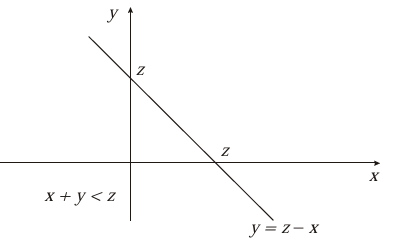
\includegraphics[scale = 0.8]{Densità di probabilità di Z.PNG}
\end{figure} 

La regione del piano x-y favorevole all'evento $F_Z (z)$ è quella al di sotto della retta 
$y = z - x$. \newline 

{
    \Large 
    \begin{equation}
        \begin{split}
            F_Z (z) 
            &=
            \iint_{x + y \leq z} 
            f_{XY} (x, y) 
            dx dy 
            \\ 
            &= 
            \int_{x = -\infty}^{+ \infty}
            \int_{y = -\infty}^{z - x} 
            f_{XY} (x, y) 
            dx dy
        \end{split}
    \end{equation}
}


Da $F_Z (z)$ è possibile ricavare $f_Z (z)$: 

{
    \Large 
    \begin{equation}
        \begin{split}
            f_Z (z) 
            &= 
            \frac{d F_Z (z)}{dz}
            \\ 
            &= 
            \frac{d}{dz}
            [\int_{x = -\infty}^{+ \infty}
            \int_{y = -\infty}^{z - x} 
            f_{XY} (x, y) 
            dx dy]
            \\ 
            &= 
            \int_{- \infty}^{+ \infty}
            f_{XY} (x, z - x)
            dx
        \end{split}
    \end{equation}
}

dove $\int_{- \infty}^{+ \infty} f_{XY} (x, z - x) dx$ è un'integrale di convoluzione. \newline 

Un caso ulteriore è quando le variabili X e Y sono statisticamente indipendenti: 

{
    \Large 
    \begin{equation}
        f_Z (z)
        = 
        \int_{- \infty}^{+ \infty}
        f_X (x) f_Y (z - x)
        dx
    \end{equation}
}

che ha, evidentemente, il significato di integrale di convoluzione tra le densità di 
probabilità dei singoli addendi. \newline 

Inoltre, possiamo ricavare valore medio: 

{
    \Large 
    \begin{equation}
        \begin{split}
            m_Z 
            &= 
            <g(X, Y)>
            \\ 
            &= 
            \int_{x = -\infty}^{\infty}
            \int_{y = -\infty}^{\infty}
            g(x, y) f_{XY} (x, y) 
            dx dy
        \end{split}
    \end{equation}
}

E anche la varianza: 

{
    \Large 
    \begin{equation}
        \begin{split}
            <\sigma_Z ^{2}> 
            &= 
            <[g(X, Y) - <g(X, Y) >]^{2}>
            \\ 
            &= 
            \int_{x = -\infty}^{\infty}
            \int_{y = -\infty}^{\infty}
            [g (x, y)  <g (x, y)>]^{2}
            f_{XY} (x, y)
            dx dy
        \end{split}
    \end{equation}
}

In particolare se $g(X, Y)$ è una somma: 

{
    \Large 
    \begin{equation}
        m_Z = m_X + m_Y
    \end{equation}
}

Il valore medio della somma di due variabili aleatorie è dunque sempre uguale alla somma dei valori medi delle varibili singole. \newline 

Inolte, sempre se esiste la somma: 

{
    \Large 
    \begin{equation}
        \sigma_Z ^{2} 
        = 
        \sigma_X ^{2} + \sigma_Y ^{2} + 2 \sigma_{11}  
    \end{equation}
}

Solo nel caso di variabili incorrelate, la varianza della somma di due variabili aleatorie è pari alla somma delle varianze delle singole variabili 
perchè $\sigma_{11} = 0$. \newline 

In questo caso particolare, possiamo scrivere anche che: 

{
    \Large 
    \begin{equation}
        C_Z (u) 
        = 
        C_X (u) C_Y (u)
    \end{equation}
} 

\newpage 

\section{Funzioni di n variabili aleatorie}

Possiamo generalizzare il caso visto in due variabili a n variabili. \newline 

{
    \Large 
    \begin{equation}
        f_{Y_1, Y_2, ..., Y_n} (y_1, y_2, ..., y_n)
        = 
        f_{X_1, X_2, ..., X_n} (x_1, x_2, ..., x_n) 
        \abs{\frac{\partial (x_1, x_2, ..., x_n)}{\partial(y_1, y_2, ..., y_n)}}
    \end{equation}
}

dove: 

{
    \Large 
    \begin{equation}
        \abs{\frac{\partial (x_1, x_2, ..., x_n)}{\partial(y_1, y_2, ..., y_n)}}
        =
        \abs{
            \det
            \begin{bmatrix}
                \frac{\partial x_1}{\partial y_1} & \frac{\partial x_1}{\partial y_2} & ... & \frac{\partial x_1}{\partial y_n} \\ 
                \frac{\partial x_2}{\partial y_1} & \frac{\partial x_2}{\partial y_2} & ... & \frac{\partial x_2}{\partial y_n} \\
                ... & ... & ... & ... \\ 
                \frac{\partial x_n}{\partial y_1} & \frac{\partial x_n}{\partial y_2} & ... & \frac{\partial x_n}{\partial y_n} 
            \end{bmatrix}
        }  
    \end{equation}
}

Sapendo la relazione tra $X_j$ e $Y_k$ pssiamo esplicitare le variabili come: 

{
    \Large 
    \begin{equation}
        X_1 = g_1 (Y_1, Y_2, ..., Y_n )
    \end{equation}
}

{
    \Large 
    \begin{equation}
        X_2 = g_2 (Y_1, Y_2, ..., Y_n )
    \end{equation}
}

... 

{
    \Large 
    \begin{equation}
        X_n = g_n (Y_1, Y_2, ..., Y_n )
    \end{equation}
}

\newpage 

\section{Teorema del limite centrale} 

Consideriamo la variabile aleatoria: 

{
    \Large 
    \begin{equation}
        Z_n = \sum_{j = 1}^{n} X_j
    \end{equation}
}


e supponiamo che le n variabili aleatorie $X_1, X_2, ..., X_n$: 

\begin{itemize}
    \item siano tra loro statisticamente indipendenti 
    \item abbiamo tutte uguale densità di probabilità $f_{X_j} (x_j) = f(x)$, con valore medio $m_{X_j} = m$ e varianza $\sigma_{X_j} ^{2} = \sigma ^{2}$
\end{itemize}

Per n che tende a $\infty$, e considerando le ipotesi scritte precedentemente, possiamo scerivere che: 

{
    \Large 
    \begin{equation}
        m_n = n \cdot m
    \end{equation}
}

{
    \Large 
    \begin{equation}
        \sigma_n ^{2} = n \cdot \sigma^{2}
    \end{equation}
}

Dalla formula di $Z_n$, definiamo questo tipo di variabile: 

{
    \Large
    \begin{equation}
        \begin{split}
            S_n 
            &= 
            \frac{Z_n - m_n}{\sigma_n}
            \\ 
            &= 
            \frac{Z_n - n \cdot m}{\sqrt{n} \cdot \sigma}
        \end{split}
    \end{equation}
}

Indipendemente da n, è chiaro che $S_n$ ha valor medio nullo e varianza unitaria. \newline 

A parte queste differenze, $S_n$ ha le stesse proprietà statistiche di $Z_n$, in particolare lo stesso andamento della densità di probabilità. \newline 

Per $n \to \infty$ è fornita dalla seguente enunciato denominato teorema-limite centrale. \newline

La densità di probabilità della variabile somma normalizzata $S_n$ tende a una variabile gaussiana con valor medio nullo e varianza unitaria; si ha cioè: 

{
    \Large 
    \begin{equation}
        \lim_{n \to \infty} f_{S_n} (s_n) 
        = 
        \frac{1}{\sqrt{2 \pi}} 
        \exp(-\frac{s_n ^{2}}{2})
    \end{equation}
}

In particolare, questo risultato asserisce che la somma di un gran numero di variabili aleatorie indipendenti segue, 
con buona approsimazione, una legge gaussiana, e ciò Indipendemente dalla particolare distribuzione di ciascuna di esse. \newline 

\newpage 

